% Options for packages loaded elsewhere
\PassOptionsToPackage{unicode}{hyperref}
\PassOptionsToPackage{hyphens}{url}
%
\documentclass[
]{book}
\usepackage{amsmath,amssymb}
\usepackage{iftex}
\ifPDFTeX
  \usepackage[T1]{fontenc}
  \usepackage[utf8]{inputenc}
  \usepackage{textcomp} % provide euro and other symbols
\else % if luatex or xetex
  \usepackage{unicode-math} % this also loads fontspec
  \defaultfontfeatures{Scale=MatchLowercase}
  \defaultfontfeatures[\rmfamily]{Ligatures=TeX,Scale=1}
\fi
\usepackage{lmodern}
\ifPDFTeX\else
  % xetex/luatex font selection
\fi
% Use upquote if available, for straight quotes in verbatim environments
\IfFileExists{upquote.sty}{\usepackage{upquote}}{}
\IfFileExists{microtype.sty}{% use microtype if available
  \usepackage[]{microtype}
  \UseMicrotypeSet[protrusion]{basicmath} % disable protrusion for tt fonts
}{}
\makeatletter
\@ifundefined{KOMAClassName}{% if non-KOMA class
  \IfFileExists{parskip.sty}{%
    \usepackage{parskip}
  }{% else
    \setlength{\parindent}{0pt}
    \setlength{\parskip}{6pt plus 2pt minus 1pt}}
}{% if KOMA class
  \KOMAoptions{parskip=half}}
\makeatother
\usepackage{xcolor}
\usepackage{color}
\usepackage{fancyvrb}
\newcommand{\VerbBar}{|}
\newcommand{\VERB}{\Verb[commandchars=\\\{\}]}
\DefineVerbatimEnvironment{Highlighting}{Verbatim}{commandchars=\\\{\}}
% Add ',fontsize=\small' for more characters per line
\usepackage{framed}
\definecolor{shadecolor}{RGB}{248,248,248}
\newenvironment{Shaded}{\begin{snugshade}}{\end{snugshade}}
\newcommand{\AlertTok}[1]{\textcolor[rgb]{0.94,0.16,0.16}{#1}}
\newcommand{\AnnotationTok}[1]{\textcolor[rgb]{0.56,0.35,0.01}{\textbf{\textit{#1}}}}
\newcommand{\AttributeTok}[1]{\textcolor[rgb]{0.13,0.29,0.53}{#1}}
\newcommand{\BaseNTok}[1]{\textcolor[rgb]{0.00,0.00,0.81}{#1}}
\newcommand{\BuiltInTok}[1]{#1}
\newcommand{\CharTok}[1]{\textcolor[rgb]{0.31,0.60,0.02}{#1}}
\newcommand{\CommentTok}[1]{\textcolor[rgb]{0.56,0.35,0.01}{\textit{#1}}}
\newcommand{\CommentVarTok}[1]{\textcolor[rgb]{0.56,0.35,0.01}{\textbf{\textit{#1}}}}
\newcommand{\ConstantTok}[1]{\textcolor[rgb]{0.56,0.35,0.01}{#1}}
\newcommand{\ControlFlowTok}[1]{\textcolor[rgb]{0.13,0.29,0.53}{\textbf{#1}}}
\newcommand{\DataTypeTok}[1]{\textcolor[rgb]{0.13,0.29,0.53}{#1}}
\newcommand{\DecValTok}[1]{\textcolor[rgb]{0.00,0.00,0.81}{#1}}
\newcommand{\DocumentationTok}[1]{\textcolor[rgb]{0.56,0.35,0.01}{\textbf{\textit{#1}}}}
\newcommand{\ErrorTok}[1]{\textcolor[rgb]{0.64,0.00,0.00}{\textbf{#1}}}
\newcommand{\ExtensionTok}[1]{#1}
\newcommand{\FloatTok}[1]{\textcolor[rgb]{0.00,0.00,0.81}{#1}}
\newcommand{\FunctionTok}[1]{\textcolor[rgb]{0.13,0.29,0.53}{\textbf{#1}}}
\newcommand{\ImportTok}[1]{#1}
\newcommand{\InformationTok}[1]{\textcolor[rgb]{0.56,0.35,0.01}{\textbf{\textit{#1}}}}
\newcommand{\KeywordTok}[1]{\textcolor[rgb]{0.13,0.29,0.53}{\textbf{#1}}}
\newcommand{\NormalTok}[1]{#1}
\newcommand{\OperatorTok}[1]{\textcolor[rgb]{0.81,0.36,0.00}{\textbf{#1}}}
\newcommand{\OtherTok}[1]{\textcolor[rgb]{0.56,0.35,0.01}{#1}}
\newcommand{\PreprocessorTok}[1]{\textcolor[rgb]{0.56,0.35,0.01}{\textit{#1}}}
\newcommand{\RegionMarkerTok}[1]{#1}
\newcommand{\SpecialCharTok}[1]{\textcolor[rgb]{0.81,0.36,0.00}{\textbf{#1}}}
\newcommand{\SpecialStringTok}[1]{\textcolor[rgb]{0.31,0.60,0.02}{#1}}
\newcommand{\StringTok}[1]{\textcolor[rgb]{0.31,0.60,0.02}{#1}}
\newcommand{\VariableTok}[1]{\textcolor[rgb]{0.00,0.00,0.00}{#1}}
\newcommand{\VerbatimStringTok}[1]{\textcolor[rgb]{0.31,0.60,0.02}{#1}}
\newcommand{\WarningTok}[1]{\textcolor[rgb]{0.56,0.35,0.01}{\textbf{\textit{#1}}}}
\usepackage{longtable,booktabs,array}
\usepackage{calc} % for calculating minipage widths
% Correct order of tables after \paragraph or \subparagraph
\usepackage{etoolbox}
\makeatletter
\patchcmd\longtable{\par}{\if@noskipsec\mbox{}\fi\par}{}{}
\makeatother
% Allow footnotes in longtable head/foot
\IfFileExists{footnotehyper.sty}{\usepackage{footnotehyper}}{\usepackage{footnote}}
\makesavenoteenv{longtable}
\usepackage{graphicx}
\makeatletter
\def\maxwidth{\ifdim\Gin@nat@width>\linewidth\linewidth\else\Gin@nat@width\fi}
\def\maxheight{\ifdim\Gin@nat@height>\textheight\textheight\else\Gin@nat@height\fi}
\makeatother
% Scale images if necessary, so that they will not overflow the page
% margins by default, and it is still possible to overwrite the defaults
% using explicit options in \includegraphics[width, height, ...]{}
\setkeys{Gin}{width=\maxwidth,height=\maxheight,keepaspectratio}
% Set default figure placement to htbp
\makeatletter
\def\fps@figure{htbp}
\makeatother
\setlength{\emergencystretch}{3em} % prevent overfull lines
\providecommand{\tightlist}{%
  \setlength{\itemsep}{0pt}\setlength{\parskip}{0pt}}
\setcounter{secnumdepth}{5}
\usepackage{booktabs}
\ifLuaTeX
  \usepackage{selnolig}  % disable illegal ligatures
\fi
\usepackage[]{natbib}
\bibliographystyle{plainnat}
\IfFileExists{bookmark.sty}{\usepackage{bookmark}}{\usepackage{hyperref}}
\IfFileExists{xurl.sty}{\usepackage{xurl}}{} % add URL line breaks if available
\urlstyle{same}
\hypersetup{
  pdftitle={Statistical Programming for the Social Sciences Using R},
  pdfauthor={Wesley Stubenbord},
  hidelinks,
  pdfcreator={LaTeX via pandoc}}

\title{Statistical Programming for the Social Sciences Using R}
\author{Wesley Stubenbord}
\date{2024-01-28}

\begin{document}
\maketitle

{
\setcounter{tocdepth}{1}
\tableofcontents
}
\hypertarget{about}{%
\chapter{About}\label{about}}

Welcome! This is the companion website for the Statistical Programming for the Social Sciences Using R course taught at Sciences Po on the Reims campus for the Spring 2024 term.

This website will contain the relevant tutorials for each week's lesson as well as other resources that you may find helpful throughout the course.

The syllabus, assignment submission portals, and other files can be found on the course Moodle site.

\hypertarget{an-introduction-to-r}{%
\chapter{An Introduction to R}\label{an-introduction-to-r}}

To get started, you will need to install two things:

\begin{enumerate}
\def\labelenumi{\arabic{enumi}.}
\item
  R, a programming language
\item
  RStudio, a software program that helps you program in R.

  \begin{itemize}
  \tightlist
  \item
    This type of software program is called an IDE, an Integrated Development Environment.
  \end{itemize}
\end{enumerate}

You don't necessarily need RStudio to program in R, but it makes life a lot easier and it's what we'll be using throughout the course.

\hypertarget{installing-r}{%
\section{Installing R}\label{installing-r}}

To install R, go to \url{https://cran.irsn.fr/index.html}, select the appropriate operating system and follow the instructions.

For example, if you have a Mac, you will click on ``Download R for macOS,'' followed, in most cases, by clicking on the ``R-4.3.2-arm64.pkg'' link beneath the ``Latest release'' header.

If you have a PC running Windows, you will click on ``Download R for Windows'' followed by ``install R for the first time'' and ``Download R-4.3.2 for Windows.''

In either case, your browser should start downloading an executable file which you will then need to run to install R.

\emph{CAUTION}: A couple of things you may need to watch out for:

\begin{enumerate}
\def\labelenumi{\arabic{enumi}.}
\item
  If you are using an older laptop, you may need to download a different version of R or RStudio. When in doubt, read the installation pages and refer to your operating system version.
\item
  If you have very little hard drive space on your computer, you may need to clear some space before you go to install RStudio. The latest RStudio version requires 215 MB and you'll need some additional space for other software and data later on in the course (around 2 GB should suffice).
\end{enumerate}

\hypertarget{installing-rstudio}{%
\section{Installing RStudio}\label{installing-rstudio}}

Once you've installed R, go to \url{https://posit.co/download/rstudio-desktop/}. Posit (a company formerly known as RStudio) offers RStudio Desktop free of charge. They also have a cloud-based version of the software (Posit Cloud) which has a free tier and paid tiers. If you have trouble using RStudio Desktop in this course, you may consider using a Posit Cloud account as discussed in the course syllabus.

Step 1 is complete - you've already installed R. On the landing page linked above, you'll find different versions of RStudio according to your computer's operating system. Select the operating system that applies to your case, download the installer, and then, once it has downloaded, run the installer from your computer and follow the on-screen steps.

If all goes well, your RStudio screen should look something like this once it is correctly installed and running:

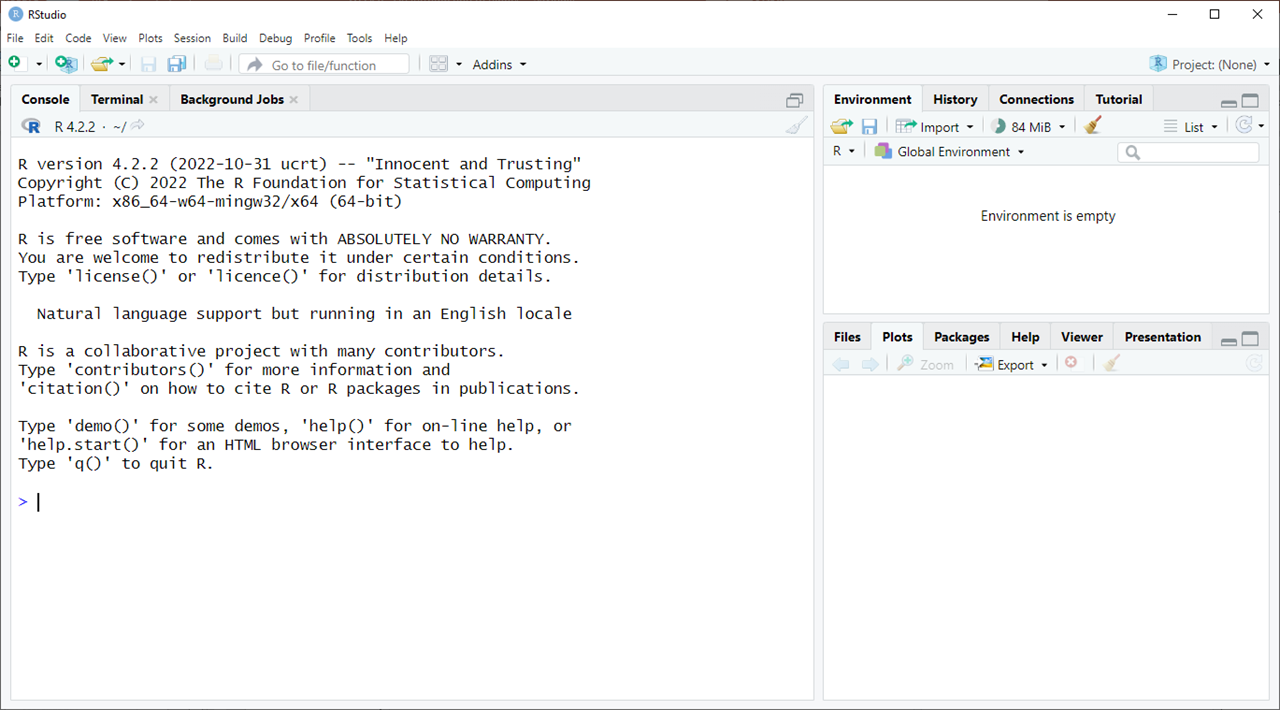
\includegraphics{docs/_main_files/figure-html/RStudio clean install.png}

On the other hand, if your screen looks like the image below, it means that you've opened the base R GUI and not RStudio. We're always going to be working in RStudio for this class, so you can close out of R GUI and open RStudio instead.

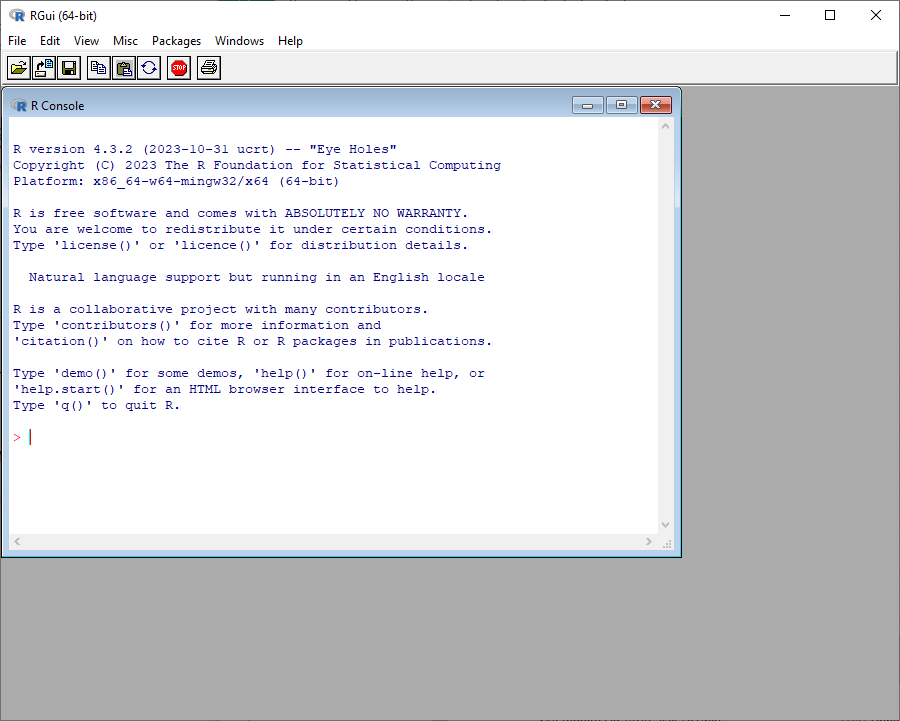
\includegraphics{docs/_main_files/figure-html/Base R GUI.PNG}

\hypertarget{using-the-console}{%
\section{Using the Console}\label{using-the-console}}

Now the fun begins. The RStudio window you've opened consists of a few different parts. The most important of these right now is the console window (highlighted below).

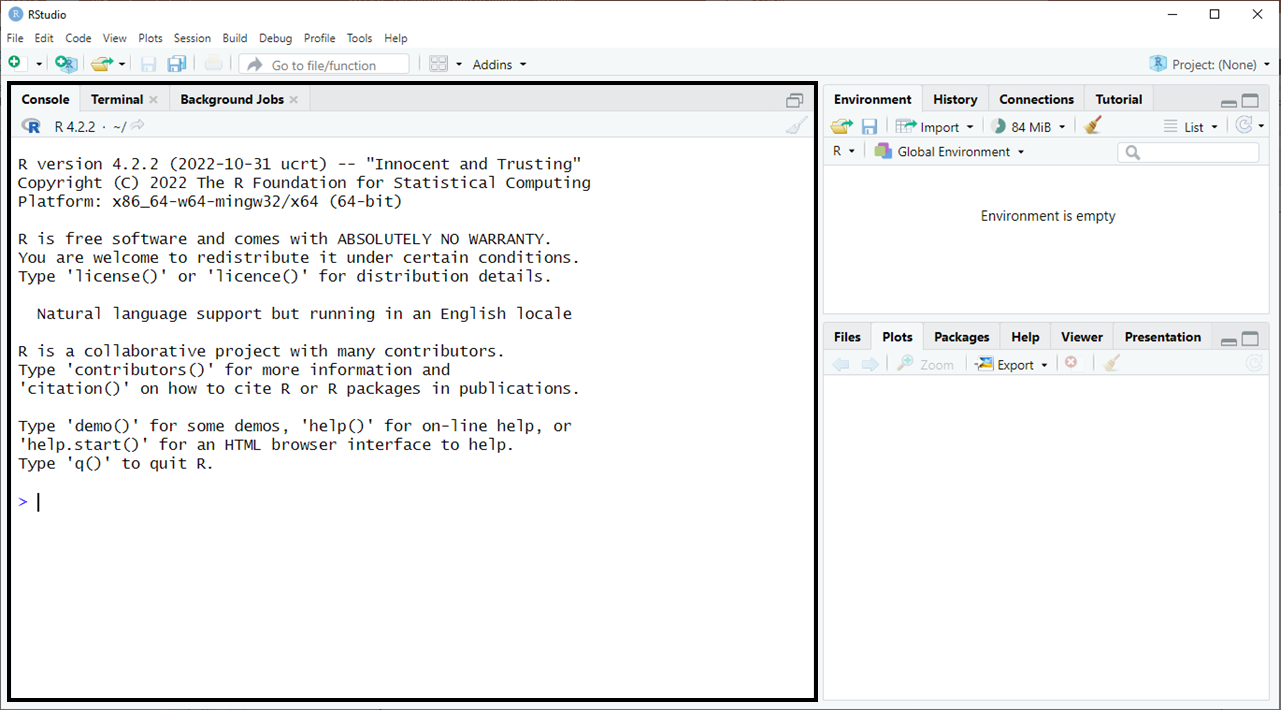
\includegraphics{docs/_main_files/figure-html/RStudio console box.png}

The console allows you to interact directly with the computer using R. So, for example, if I want to use R as a calculator, I can type in the following in the console and obtain a result:

\begin{Shaded}
\begin{Highlighting}[]
\DecValTok{1}\SpecialCharTok{+}\DecValTok{1}
\end{Highlighting}
\end{Shaded}

What happens when you press enter? You get something like this:

\begin{Shaded}
\begin{Highlighting}[]
\DecValTok{1}\SpecialCharTok{+}\DecValTok{1}
\end{Highlighting}
\end{Shaded}

\begin{verbatim}
## [1] 2
\end{verbatim}

In other words, you've provided an \textbf{\emph{input}}, 1+1, and received an \textbf{\emph{output}}, 2. The first number {[}1{]} in brackets indicates the number of the line of output. This is particularly helpful when you are running a complex bit of code, but it's important not to confuse it with the output.

Try entering a few more inputs, such as:

\begin{enumerate}
\def\labelenumi{\arabic{enumi}.}
\item
  10/3
\item
  (10/3) + 1
\item
  (10/3) + 1 + (5.111)\^{}2
\end{enumerate}

R is able to handle basic math operations with ease. What about other operations? Can R accept variables?

Try this:

\begin{Shaded}
\begin{Highlighting}[]
\NormalTok{x }\OtherTok{=} \DecValTok{1}
\end{Highlighting}
\end{Shaded}

What happens when you press enter? What happened to the output?

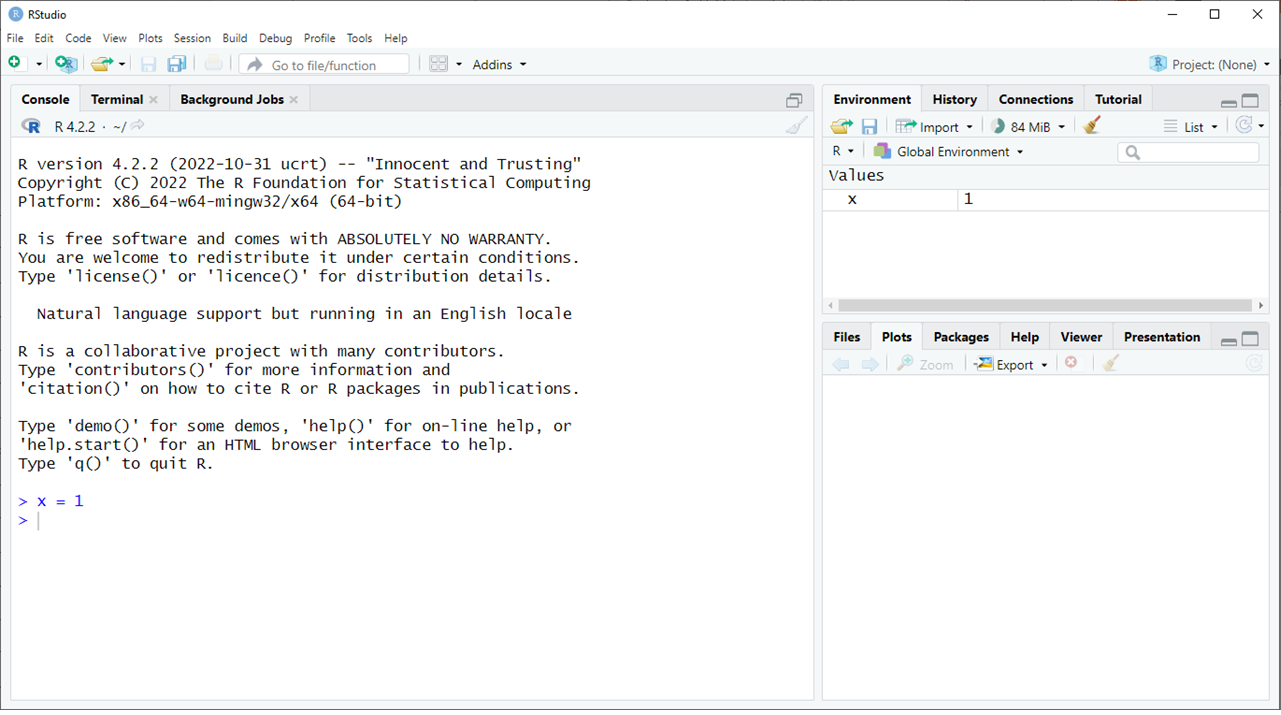
\includegraphics{docs/_main_files/figure-html/RStudio console_x1.png}

The trick here is that there is no output. You've stored a value, 1, in a variable, x, somewhere in your computer's memory or in what we might call the environment. RStudio shows you this in the Environment window in the top right.

We can recall the value we input into our variable, x, by entering just the variable name in the console.

\begin{Shaded}
\begin{Highlighting}[]
\NormalTok{x}
\end{Highlighting}
\end{Shaded}

\begin{verbatim}
## [1] 1
\end{verbatim}

See! R remembers what you stored in your environment.

Try the following:

\begin{enumerate}
\def\labelenumi{\arabic{enumi}.}
\item
  Can you assign a new value to your variable x?
\item
  Can you perform math operations on a variable (e.g., x*2)?
\item
  Can you create a new variable, y, and use it in math operations with x (e.g., x * y)? What might you have to do with y first?
\item
  Can you change the type of variable? What if, for example, I don't want x = 1, but I want x to be equal to the word ``apple''?
\end{enumerate}

\hypertarget{variables}{%
\section{Variables}\label{variables}}

If you've made it this far, congrats! Here's another thing you can try. Enter the following in the console:

\begin{Shaded}
\begin{Highlighting}[]
\NormalTok{x }\OtherTok{\textless{}{-}} \FunctionTok{c}\NormalTok{(}\DecValTok{1}\NormalTok{,}\DecValTok{2}\NormalTok{,}\DecValTok{3}\NormalTok{,}\DecValTok{4}\NormalTok{,}\DecValTok{5}\NormalTok{)}
\end{Highlighting}
\end{Shaded}

You'll notice, we're using a different operator here. It's a less than symbol (\textless) followed by a dash (-). This is called an \textbf{assignment operator}. It has the same function as the equals sign (=) and you can use either. I just so happen to prefer the way this one looks.

What happens when you press enter? You have created a \textbf{vector}. Like other types of variables in R, a vector is an object. A vector holds a set of values of the same type. In this case, the vector x is holding a set of numbers.

We can do all sorts of things with vectors and other objects in R. We can, for example, find the sum of a vector.

\begin{Shaded}
\begin{Highlighting}[]
\FunctionTok{sum}\NormalTok{(x)}
\end{Highlighting}
\end{Shaded}

\begin{verbatim}
## [1] 15
\end{verbatim}

How did we get an output of 15? 1+2+3+4+5 = 15. We can also find the mean of a vector.

\begin{Shaded}
\begin{Highlighting}[]
\FunctionTok{mean}\NormalTok{(x)}
\end{Highlighting}
\end{Shaded}

\begin{verbatim}
## [1] 3
\end{verbatim}

And we can perform other operations. Try the following:

\begin{enumerate}
\def\labelenumi{\arabic{enumi}.}
\item
  Can you find the median of the vector x? What about the mode?
\item
  What happens when you multiply a vector?
\item
  Can you create a new vector which consists only of letters?
\end{enumerate}

\hypertarget{saving-your-work}{%
\section{Saving Your Work}\label{saving-your-work}}

As you've begun to see, working with a scripting language like R is quite different from working with software like Microsoft Excel or Google Sheets. You work interactively with data using code rather than by changing values directly in a user interface.

One of the great benefits of interacting in this way, particularly for the social sciences, is that it allows others to fully reproduce your work. If they have your code, they can repeat the exact same steps you took.

Think about it this way: when you change a value in a cell in an Excel spreadsheet, will someone else know what was in that cell before you changed it? No.

In R, however, we can leave the source data alone and save the code we use to manipulate it. Now others can see exactly what you've done to each value and reproduce your analysis.

There are a couple of different ways of saving your code:

\begin{enumerate}
\def\labelenumi{\arabic{enumi}.}
\item
  In an R Script file, which is a simple text file containing only your code
\item
  In an R Markdown file, which is basically an interactive notebook that allows you to see your code and the results next to each other
\end{enumerate}

We're going to start with an R Script file and try out R Markdown later on.

\hypertarget{creating-and-saving-r-script-files}{%
\section{Creating and Saving R Script Files}\label{creating-and-saving-r-script-files}}

To create an R Script file in RStudio, go to File \textgreater{} New File \textgreater{} R Script.

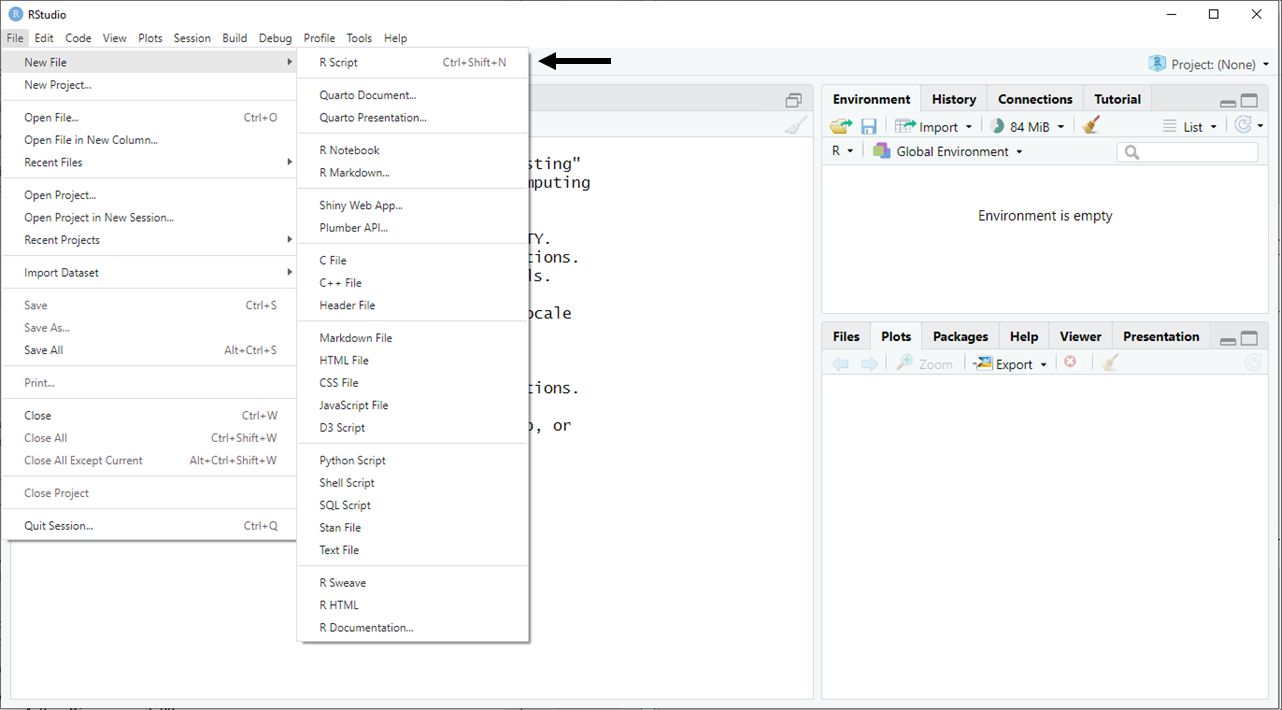
\includegraphics{docs/_main_files/figure-html/RStudio_Opening an R Script File.png}

You should now have a window open in RStudio which looks like this:

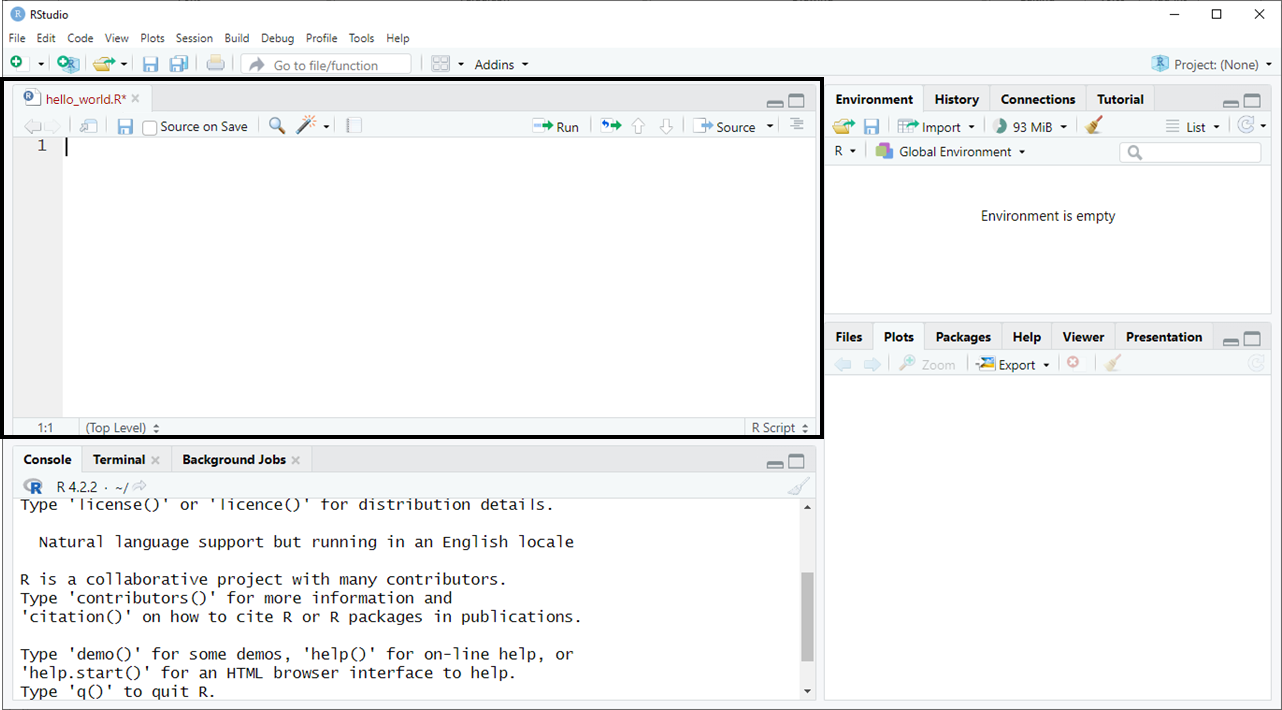
\includegraphics{docs/_main_files/figure-html/RStudio_Opened RScript.png}

You can enter comments in your R Script file using a hash tag (\#) at the beginning of each comment line. A hash tag lets R know that this line should not be run as code.

I like to add my name, the date, and a description to each file I use. I'll ask that you use a header for each R file you submit for this class as well.

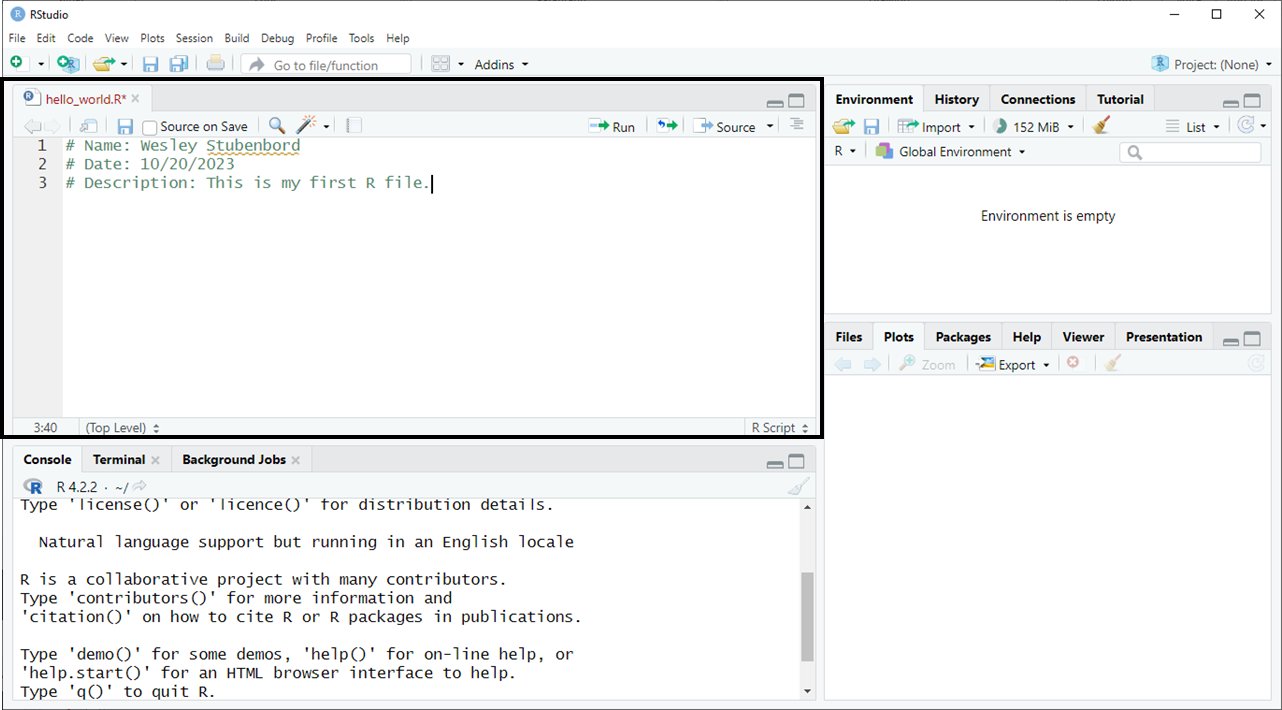
\includegraphics{docs/_main_files/figure-html/RStudio_Commenting in an R Script file.png}

Now, save your R Script somewhere on your computer. Go to File \textgreater{} Save As, choose a safe place on your computer to store it (I recommend creating a folder for this course), give it a name, and then press save. I called mine ``hello\_world''.

\hypertarget{interacting-with-an-r-script}{%
\section{Interacting with an R Script}\label{interacting-with-an-r-script}}

Interacting with an R Script is slightly different from interacting in the console. Now when you type in code and hit enter, it will not execute the code, it just creates a new line in your file.

To run code in a script either:

\begin{enumerate}
\def\labelenumi{\arabic{enumi}.}
\tightlist
\item
  Select the lines you wish to run with your cursor and then press \textless Ctrl\textgreater{} + \textless Enter\textgreater{}
\item
  Or, put your cursor on the line you wish to run and click the Run button in the top right of the R Script file window
\end{enumerate}

The first option allows you to run multiple lines at a time and the second runs only the line you are currently on. The results of your code will appear in the console window below your R Script file when run successfully.

After you finish modifying your R Script file, you can save it and close out of R Studio. The next time you wish to access your saved code, you can open your R Script file and it will be exactly as you left it.

  \bibliography{book.bib,packages.bib}

\end{document}
